\documentclass[conference]{IEEEtran}
\usepackage{graphicx}
\usepackage{amsmath}
\usepackage{booktabs}
\usepackage{cite}

\begin{document}

\title{Local Search, Adversarial Search and Constraint Satisfaction:\\
N-Queens, Tank Battle and Kakuro}

% Fill in the real names and student IDs. The lecturer is the last author.
\author{\IEEEauthorblockN{Member A, Member B, Member C, Member D, Nguyen Thanh An}
\IEEEauthorblockA{Faculty of Information Technology, Ton Duc Thang University\\
Ho Chi Minh City, Vietnam}}

\maketitle

\begin{abstract}
TODO (write last, after all results are final). Summarise in 4--6 sentences: the three tasks,
the main method of each task, the most important experimental result of each task,
and what was completed.
\end{abstract}

\section{N-Queens: Propositional Logic and Local Search}
% Section written by A and B (requirements 1.1, 1.2, 1.3).

\begin{figure}[t]
\centering
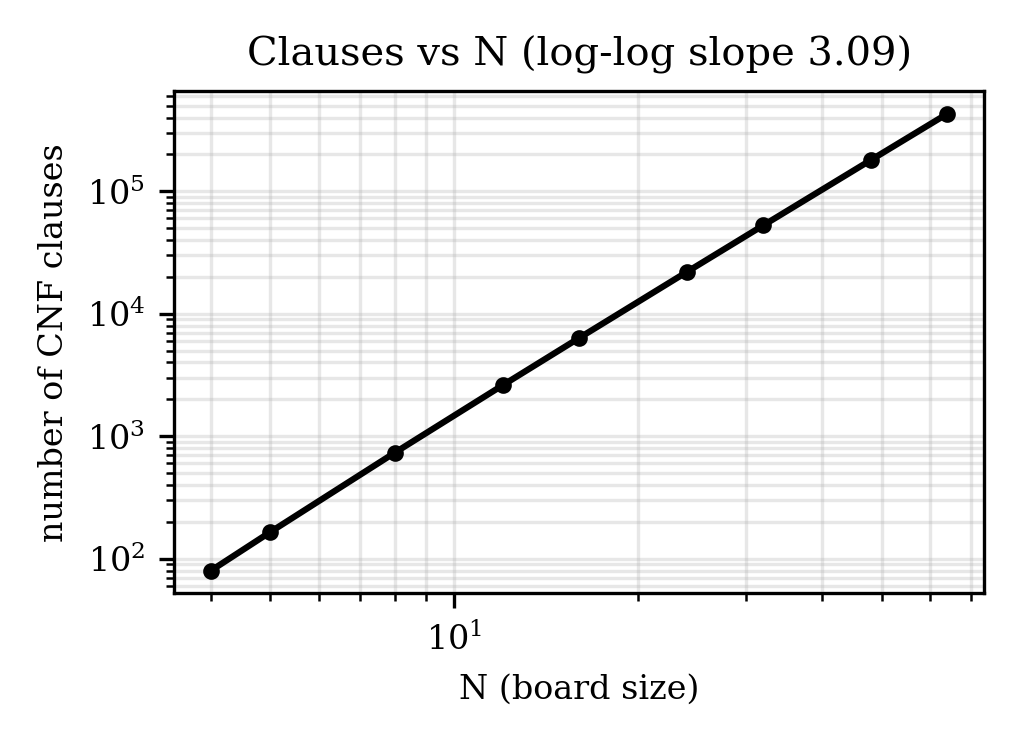
\includegraphics[width=\columnwidth]{figures/sat_clauses.png}
\caption{Number of CNF clauses against board size $N$ (log-log scale).}
\label{fig:clauses}
\end{figure}

\begin{figure}[t]
\centering
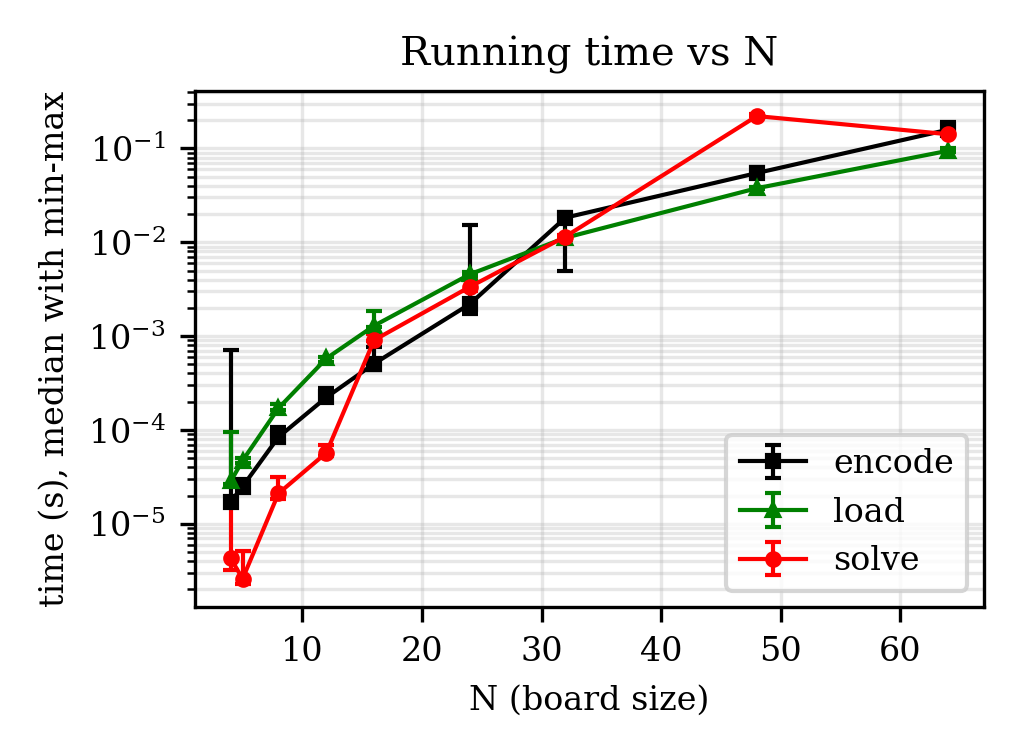
\includegraphics[width=\columnwidth]{figures/sat_time.png}
\caption{Encoding, loading and solving time against $N$. Points are medians of five runs,
bars show minimum and maximum.}
\label{fig:time}
\end{figure}

\section{Tank Battle: Adversarial Search}
\subsection{Zero-Sum Game Formulation}
Tank Battle is played by two players, MAX (tank~1) and MIN (tank~2). Both players see the whole
board and nothing is random, so the game is a deterministic, perfect-information zero-sum game:
whatever one side wins, the other side loses. We use the six components of a game from~\cite{aima}.

\textit{State.} A state holds the walls that are still standing (each with its HP), the position,
facing direction and HP of both tanks, the HP of both bases, the bullets in flight (at most one per
tank), the number of cycles played, and the action MAX has already chosen in the current cycle.

\textit{Players.} A cycle is split into two plies. MAX chooses first and its action is kept
aside. MIN then chooses, and only after that are both actions applied together. This turns a
simultaneous game into a turn-taking one, so Minimax can be used. Because MIN sees MAX's action,
the value computed by Minimax is a worst-case value for MAX.

\textit{Actions.} Six actions are always available: MOVE\_UP, MOVE\_DOWN, MOVE\_LEFT, MOVE\_RIGHT,
FIRE and STAY. An action that cannot be carried out (walking into a wall, firing while a bullet is
already in flight) is handled by the rules and not forbidden, so the branching factor is always
$b=6$ per ply.

\textit{Transition.} After the MIN ply, one cycle is processed in a fixed order: tanks move, new
bullets are created, then every bullet flies up to three cells, one cell at a time. After each cell
the bullet is checked against walls, tanks and bases. On a hit it removes 1 HP from the target and
disappears. Two tanks moving into the same cell both stay where they are.

\textit{Terminal test and utility.} The game ends when a tank or a base reaches 0 HP, or after a
fixed number of cycles. The utility for MAX is $+1$ for a win, $-1$ for a loss and $0$ for a draw
(both sides lose in the same cycle, or the cycle limit is reached).

\subsection{Applying the Search Algorithms}
Minimax searches down to terminal states and backs up the maximum at MAX nodes and the minimum at
MIN nodes. With $b=6$ and depth $m$ plies it visits about $6^m$ states, so it is only practical on
small maps or for very short games. Alpha-Beta pruning returns the same value and the same move but
skips branches that cannot change the decision. Heuristic Minimax stops at a depth limit and uses an
evaluation function instead of the utility. Our evaluation function combines the tank HP
difference, the base HP difference, which side has a clear line of fire, and the distance to the
enemy base. Terminal states are scored $\pm 1000$ so that a real win always ranks above any
estimate. Heuristic Minimax can also be combined with Alpha-Beta pruning.

% Subsections 2.2 (experiments) and 2.3 (GUI and agent loading) are written by D and B.

\section{Kakuro: Constraint Satisfaction}
% Section written by D (3.1, 3.2) and A (3.3).

\section{Contributions}
% Table: member, tasks done, completion level (0--100\%). Agreed by the whole group in week 5.

\section{Self-evaluation}
% Table: task, self-estimated score.

\section{Conclusion}
% Write last: requirements, approaches, results, levels of completion.

\begin{thebibliography}{1}
\bibitem{aima} S. Russell and P. Norvig, \textit{Artificial Intelligence: A Modern Approach}, 3rd ed.
Upper Saddle River, NJ, USA: Prentice Hall, 2009.

\bibitem{pysat} A. Ignatiev, A. Morgado, and J. Marques-Silva, ``PySAT: A Python toolkit for
prototyping with SAT oracles,'' in \textit{Proc. Int. Conf. Theory and Applications of
Satisfiability Testing (SAT)}, 2018, pp. 428--437.

\bibitem{kakuro} ``Kakuro,'' Wikipedia. [Online]. Available: https://en.wikipedia.org/wiki/Kakuro
\end{thebibliography}

\end{document}
